\begin{example} \label{Ex:3.2.Eg7}
Sketch $\ds f(x) = \frac{5(x-2)(x+1)}{x^2+2x+4}.$

\solution We again follow the steps outlined in the Curve Sketching Concept.
\begin{enumerate}[1)]
\item We assume that the domain of $f$ is all real numbers and consider restrictions. The only restrictions come when the denominator is 0, but this never occurs. Therefore the domain of $f$ is all real numbers, $\mathbb{R}$.
\item We find the critical values of $f$ by setting $\fp(x)=0$ and solving for $x$. We find 
$$\fp(x) = \frac{15x(x+4)}{(x^2+2x+4)^2} \quad \Rightarrow \quad \fp(x) = 0 \text{ when } \ x=-4,0.$$
\item We find the possible points of inflection by solving $\fpp(x) = 0$ for $x$. We find
$$\fpp(x) = -\frac{30x^3+180x^2-240}{(x^2+2x+4)^3} .$$ The cubic in the numerator does not factor very ``nicely.'' We instead approximate the roots at $x= -5.759$, $x=-1.305$ and $x=1.064$.
			
\item There are no vertical asymptotes.
\item We have a horizontal asymptote of $y=5$, as $\ds \lim_{x\to-\infty}f(x) = \lim_{x\to\infty}f(x) = 5$.
\item We place the critical points and possible points on a number line as shown below and mark each interval as increasing/decreasing, concave up/down appropriately.
	
\begin{center}
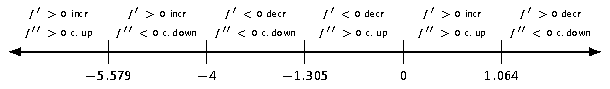
\includegraphics[scale=.75]{figures/figsketchline3}
\end{center}
	
\item In Figure~\ref{fig:sketch3}-(a) we plot the significant points from the number line as well as the two roots of $f$, $x=-1$ and $x=2$, and connect the points with straight lines to get a general impression about the graph. In Figure~\ref{fig:sketch3}-(b), we add concavity. Figure~\ref{fig:sketch3}-(c) shows a computer generated graph of $f$, affirming our results.		
\end{enumerate}
\end{example}

\begin{marginfigure}[-4cm] % MARGIN FIGURE
%\captionsetup[subfigure]{labelformat=empty}
\subfloat[]{\margingraphics{figures/figsketch3a}}

\subfloat[]{\margingraphics{figures/figsketch3b}}

\subfloat[]{\margingraphics{figures/figsketch3}}
\caption{Sketching $f$ in Example~\ref{Ex:3.2.Eg7}.}
\label{fig:sketch3}
\end{marginfigure}